\section{Control system architecture}
\label{sec:Chap3-ControlSystemArchitecture}
Chapter~\ref{chap:phasenoisepaper} sets the general background to double-Fourier interferometry when used mostly in spectroscopy mode. It sets the mathematical formalism to estimate the spectral sensitivity, given various sources of gaussian noises. 

In this section, we see more directly how this applies to BETTII, and how the system is designed to satisfy these requirements in order to guarantee good observations.

\subsection{Overall strategy}

\subsubsection{Requirements}
The strategy that we developed aims at satisfying the requirements established in the previous section, under the cost, time and personnel constraints that we were subject to. It fundamentally relies on the fact that \textit{knowledge} is more important than \textit{control}. While several research groups [CITE WASPS] are attempting to provide sub-arcsecond balloon gondola control, we are not going to. This strategy uses the fundamental advantage that the interferometer has over traditional pointed observatories: the decoupling of the phase with the pointing. This feature of interferometers refers to the possibility of obtaining electromagnetic interference even when the telescopes are slightly mispointed from the target. 

There three levels of requirements for our instrument to produce interferograms. First, both arms need to be pointed at the target, so that an image of the target seen through each arm is formed at the detector. For our purpose this will largely be set by the limitation of the field of view of the instrument, which is about 2 arcminutes. When a target is not exactly on-axis with the telescope, it can still fall on the detector if tip/tilt correction happens downstream. The tip/tilt correction will create aberrations, but these are relatively well behaved at our wavelengths. Hence, this requirement can be expressed as an overall pointing requirement of the instrument to some amount that can be corrected in tip/tilt in each individual arms. We set this to $\pm$~15". This also roughly corresponds to one single pixel on the short band detector, and half a primary beam's FWHM.

Once the instrument is pointed to the desired target to within $\pm$~15", there needs to be a fine guiding system in each arm that allows for the remaining correction. This level of control needs to overlap the beams to a small fraction of a pixel to get maximum overlap and minimum visibility losses. We set this requirement to 1.5" r.m.s., which corresponds to a tenth of a pixel's size. The fine guidance system needs to operate over a range of at least $\pm$~15" to pick up where the previous level of requirements stops. It also needs to happen with high bandwidth to ensure that only minimum motion is occurring at timescales comparable to a data acquisition timescale. This system is described in section [].

Finally, an angular mispointing of the baseline vector with respect to the target can be might still exist, even if both beams are overlapped properly. This introduces an unwanted optical delay that can push the fringe packets outside our nominal OPD scanning range. Control of this optical delay is critical for interferometry, as it is required to properly reconstruct the OPD axis of the interferograms that are the elementary data blocks of the instrument. This can be achieved using a delay line . This is commonly done for all interferometers on the ground [CITE], and we will implement a device like this on BETTII as well [section]. For this to work, we need to be able to monitor the changes in OPD accurately, which is equivalent, on short timescales, to accurately estimate the attitude of the payload.

A good estimate of the attitude of our payload can lead to an accurate angular difference between our baseline vector and our target. This angular difference can be converted to an OPD using simple geometric arguments, and can then be fed to the delay line for correction. With an 8~m baseline length, an mispointing of 1" along the baseline direction corresponds to an OPD of about 40$\um$, or one full wavelength of BETTII's short-wavelength band. In order to produce quality interferograms, we will need to know the OPD to a fraction of this [SEE previous section]. 


\subsubsection{The PID control loop}

Before we elaborate on the control architecture of the entire system, let's first discuss the elementary controls block: the PID.

A Proportional-Integral-Derivative (PID) control loop is one of the most basic, yet most used method to build systems with active control. The problem that these systems try to solve is simply to make an object reach a desired state: a sensor is used to measure the current state, and the difference between the desired state and the current state is fed to an apparatus capable of changing the state. Most commonly, this uses motors and either position or velocity sensors, but it can also be used for example for temperature control in a cryogenic environment, where heaters are used to change the temperature. For simplicity, in the rest of this work, we will always consider a loop with sensors and actuators. 

In its most simple expression, the PID can be reduced to a simple proportional loop. That is, the command is proportional to the error between the desired and measured state. The value of this proportional coefficient usually sets the dynamics of the response, as a large proportional gain $\Kp$ will mean that even a small deviation from our desired state will trigger a large response. Sometimes, a purely proportional system can lack stability.

A proportional-derivative loop adds the information of the speed at which the error varies. If the error is growing quickly, we can increase our command. If the error is being reduced quickly, it is time to slow down the command to avoid overshooting our target. This uses the time derivative of the error that multiplies a gain, $\Kd$, and has the effect to damp the motion. A PD loop usually will help with the system's stability.

But even then, a proportional-derivative does not guarantee that you will reach your desired state. We then complete the PID loop with an integral gain $\Ki$, which multiplies the integral of the error over some length of time. While the $\Kp$ and $\Kd$ gains mostly control the dynamics of the response, the integral term will control the steady-state error and ensure it converges to zero. While useful, this term needs to be considered with precaution, as some situations can lead to a diverging response.

\begin{figure}[!ht]
	\centering
	\includestandalone{Figures/SimplePID}
	\caption{}
	\label{fig:SimplePID}
    \end{figure}



A simple PID loop diagram is shown in Fig~\ref{fig:SimplePID}, with the desired input state at the entrance of the loop and the real state at the output of the loop. It is often the case that the state cannot be directly measured: this require the use of an \textit{estimator} or \textit{observer}, in which various indirect measurements will feed a mathematical model of the system to estimate its parameters. The relevant example for us is a scenario where we only measure a velocity measurement, while we want to close the loop on the position. Simply put, we know that the position has an integral relationship with the velocity, and the observer's role is to estimate the integration constants.

The estimator is also used to realize \textit{sensor fusion}. This consists of combining various types of measurements to provide the best estimate of the state to feed back to the control loop. The various measurements often happen at different discrete rates, with different lag times, which can lead to rather complex implementations. One of the most well-known estimation algorithms is the Kalman filter, which we will discuss at length in Section []. 

For BETTII, each subsystem has its own PID control loop. Each PID loop structure consists of 7 variables: the $\Kp$, $\Kd$, $\Ki$ gains, and overall scaling factor, an upper and a lower limit on the command, and a boolean value that is used to reset the content of the integral term used to multiply $\Ki$. 

\subsubsection{Control loop design}

The three levels of control that we need are:
\begin{enumerate}
\item Coarse control of the entire gondola to within $\pm~15$",
\item Fine pointing control of each beam to 1.5" r.m.s.,
\item Fine knowledge of the attitude to $\approx 0.15"$ r.m.s., followed by appropriate OPD control
\end{enumerate}

At its fundamental level, the problem is to implement a system that satisfies these requirements, starting with only the target's location in right ascension (RA) and declination (DEC). Ideally, the system needs to be able to achieve these goals autonomously. All of the operating modes follow from this.

All of the pointing will be done in the reference frame of the gondola, which is tied solidly to the reference frame of the gondola (nominally they are the same) and the star cameras (nominally off by -45~degrees about the $\vectors{y} axis$. In the following sections, we describe how the inertial attitude of the gondola is determined. Once it is known, a target's RA and DEC can be converted to a desired local azimuth $\Az$ and elevation $\El$ in the spherical coordinates attached to the gondola reference frame (see Fig.~\ref{fig:AzEl}). It is important to note that when we mention "azimuth", we are not referencing to any cardinal directions, as it can be done for other applications. For us, an azimuth is one of the two spherical angles that describe the position of our target in the current gondola reference frame. Note that the elevation angle is defined as being zero in the ($\vectors{x}_\gyros$,$\vectors{y}_\gyros$)-plane.

\begin{figure}[!ht]
	\centering
	\includestandalone{Figures/AzEl}
	\caption[Azimuth and elevation of a target]{}
	\label{fig:AzEl}
    \end{figure}


Once the turbulence from the ascent have died out, the control system starts to determine where the gondola is currently pointing using the star cameras. For the software to process the star camera image, the payload has to be still to avoid blurring of the stars on the CCD. Hence, the first order of business is to slow down the payload's inertial velocity, which is measured by the gyroscopes. This is also called $\BRAKE$ mode.

The first time the system receives a star camera frame and identifies its inertial position, this triggers the estimator algorithm that constantly combines gyroscope and star camera information. From this point on, we have a reasonable estimate of where we are pointed in the inertial frame at all times. When a new target in RA and DEC is set by the flight computer, the system will enter the $\SLEW$ mode. This creates a profile of azimuth position and velocity


\begin{figure}[!ht]
	\centering
	\includestandalone{Figures/ControlSystem}
	\caption[Control System Design]{}
	\label{fig:ControlSystem}
    \end{figure}


\subsection{Coordinate systems}


\begin{figure}[!ht]
	\centering
	\includestandalone{Figures/BETTII_coordinate_system}
	\caption[BETTII coordinate systems]{}
	\label{fig:CoordinateSystem}
    \end{figure}

    
%     \begin{figure}[!ht]
% 	\centering
% 	\includestandalone{Figures/starCameraRefFrame}
% 	\caption{Star camera angles. The star camera reference frame as well as the telescope reference frame are represented here with the celestial sphere local RA and DEC axes in the background. There is a known matrix that transforms the star camera reference frame, where inertial attitude is measured, to the telescope reference frame, where error vectors are computed. The error vector is determined on the plane of the sky and has two projections on the telescope reference frame. The $\Delta\El=\Delta$El component corresponds to the elevation error and is corrected by the siderostat angle. The $\Delta\xEl=\Delta$xEl component corresponds to the cross-elevation error, and is corrected by the CCMG gimbal angle. Note that as the siderostat elevation is adjusted to reduce the elevation error, the transformation matrix between the star camera and telescope reference frames is adjusted as well.}
% 	\label{fig:starcamRefFrame}
%     \end{figure}


\begin{figure}[!ht]
	\centering
	\includestandalone{Figures/CelestialSphereRAandDEC2}
	\caption[The celestial sphere]{}
	\label{fig:celestialSphere}
    \end{figure}

\begin{figure}[!ht]
	\centering
	\includestandalone{Figures/starCameraRefFrame}
	\caption[The star camera reference frame]{}
	\label{fig:starcamRefFrame}
    \end{figure}

\subsection{Modes of operation}

Make table with all modes; from launch to obtaining fringes

The payload has several modes of operation which are used in the various phases of a flight.


\subsection{Subsystems}



\subsection{Gyroscopes}

We purchased three SRS-2000 fiber-optic gyroscopes from Optolink. This gyroscope technology uses the Sagnac effect and is the cutting edge in inertial rotational velocity measurements \citep[for a review of the state-of-the-art see, \textit{e.g.}][]{ElBadaoui:2014fr}. We chose these devices for their incredibly low angular random walk, which is a measure of their inherent noise. If we were to trust the gyroscope measurement and integrate its velocity to obtain a position estimate, the estimation error we would make after 1 hour of integration has a standard deviation of about 2 arcseconds.

The devices have a bandwidth of 50~Hz, but can be triggered at up to 2000~Hz. Their extreme stability is contingent upon proper temperature stabilization, which is done with a closed-loop set at their calibration temperature of 23.5$^{\circ}\pm 0.5$~C using an active built-in Peltier element. This Peltier element transforms electric power into either heating or cooling \citep{Peltier:1834vu}.

However, their sensitivity has complicated some of their testing. As soon as we attach a gyroscope to any structure, it measures its vibrational modes, which makes it hard to make a stable measurement of the gyroscope's drift stability. This includes the vibrations that are inherent to the building in the which they are placed.

We were successful at measuring the gyroscopes over long periods of time by attaching them flush to a heavy slab of metal, and putting the slab of metal flush on the floor of one of NASA Goddard's optics labs in building 34. These floors are especially made to isolate the room from vibrations.

We proceeded to an identical series of tests for each gyroscope:
\begin{enumerate}
\item We acquired data at 2000~Hz for N minutes to measure a proper power spectral density and characterize the noise;
\item We acquired data at 100~Hz for $\sim$ 8 hours to study the drift properties.
\end{enumerate}

The properties that we are looking for are typical instantaneous angular random walk, and the overall drift of the gyroscope's mean. When the gyroscopes are set on the floor, they measure a component of the Earth's rotation vector in inertial space. The mean of the measurement depends on the exact angle at which the device is placed with respect to the zenith vector, and is of no importance for this noise study. We seek to understand how much the mean varies over long periods of time. To avoid disturbances from the building vibrations (opening/closing of doors, etc), we operated entirely after regular working hours.

Table of gyro specs and measurements for each gyro

\subsubsection{Normality tests}
First and foremost, we wanted to study the gyroscope's noise statistical distribution. We ran a few standard normality tests on chunks of the 8-hour data for each gyroscope. While the tests on individual small chunks of data never reject the null hypothesis (that the distribution is normal), the distribution of the total 8 hours does with a very high probability, using both the Anderson-Darling and the Kolmogorov-Smirnov test.

Since the data is always consistent with being normally distributed over timescales of tens of minutes, after close inspection of the long-term quartile plots and histograms, we determined that it would be safe to consider the distribution as normal for the purpose of our attitude estimator. 

It is important to note that in their factory settings, the gyroscopes' noise distribution was not normal at all. It exhibited electronic peaks with many harmonics, at frequencies that were varying as a function of the gyroscope inclination. After talking to the manufacturer, we determined that it was caused by the closed-loop algorithms inside the gyroscope electronics. The problem was known by them, and the remedy was to inject a random phase perturbation in the closed loop. This had the effects to get rid of those frequency peaks, at the cost of increasing the overall noise variance by a factor of 4. The noise levels that are specified by the company are very close to the noise seen when using that random phase modulation. Hence, if one does not care as much at the frequency content of the gyroscope, it is possible that this device could work even much better than it does for us.

\subsubsection{PSD and Allan variance}

The usual frequency-domain analysis tool is the power spectral density (PSD). This allows us to spot any frequency peaks in the data, and let us look at the $1/f$ noise behavior, which the typical low-frequency behavior that indicates drifts in the signal. The 100~Hz data is all we need, as the gyroscope's bandwidth is 50~Hz. Hence, the 2000~Hz data does not contain any more information than the 100~Hz. In fact, while plotting the PSD of the 2000~Hz data, we can see clearly the break at 50~Hz characteristic of a 50~Hz low-pass filter.

Another common tool to study of the gyroscope's performance is to plot the Allan variance. The Allan variance gives a time-domain analysis of the gyroscope's noise that is complementary to the power spectral density.

\subsection{Star cameras}



\subsection{Azimuth control (CCMG)}

The CCMG features multiple encoders and motors. First, there is a brushless DC motor that spins each wheel, with a relative 13-bit encoder that monitors where the wheel is in its rotation. Second, there is a Beckhoff AS1050 stepper motor that controls the wheels' shaft angle. On the gimbal, there is a 13-bit  absolute magnetic encoder that measures the angle of the wheels from some reference. 

The motion controller that we use to monitor the wheel's speed is a brushless-DC Galil motion controller DMC-4020. It reads out the wheel encoders and controls the current to the wheels accordingly. It directly, independently implements the closed-loop system of the wheels, including all of the gains, acceleration/deceleration, and jogging speeds associated with the desired motion.

The motion controller was modified to accept an external clock pulse in order to synchronize the wheels' motion with our master clock signal. It requires a clock pulse at 1.024~kHz, and deviations from this value will require changing some of the gains - it is our understanding that the controller uses a 1.024~kHz crystal oscillator to generate it's time basis, as some of the gains and parameters to the controller can directly be entered as, for example, "steps per second". 

At power-up, the wheels immediately start accelerating to their cruising speed of 3000~rpm. They take about 10 minutes to reach their target. The wheels' frequency is set for the entire duration of the flight.

The gimbal is controlled with another Galil Motion controller, a 2-axis stepper driver DMC-4020, which can also be synchronized with an external clock. Only one axis is used for the CCMG, while the second axis is used by the momentum dump motor (see section~\ref{subsec:chap3momdumpmotor}). The controller operates in micro-stepping mode and has a very smooth response, in contrast to previous controllers we tested which create a lot of vibrations. The controller is set always to use 64 micro-steps per step, and the motor is a [REFERENCE] with 200 steps per revolution. The motor is outfitted with a Beckhoff AG1000 planetary gearhead with a 3.7:1 reduction ratio. The gearbox itself has a ratio of 25, which creates a total gear ratio of 92.5. Hence, a 360$^\circ$ revolution of the stepper corresponds to $360/92.5=3.9^\circ$ motion of the shaft. A motion of 1$^\circ$ of the shaft correspond to 3889 motion controller steps. A motion of 90$^\circ$ of the shaft correspond to 296000 motion controller steps. Finally, the same 90$^\circ$ motion will translate to a 2048 step change in the gimbal magnetic encoder.

In practice, all of the control is done using the regular stepper motor encoder. The magnetic encoder is used for limit-checking and to feed back to the momentum dump mechanism. With this in mind, we can now relate the control signal (stepper motor micro-steps per second) to the physical torque that the wheels provide. 
\begin{eqnarray}
\Delta\theta\units{rad} &= &\frac{2\pi}{92.5\times 200\times 64}\Delta(\textrm{micro-steps}) \\ 
& \sim & 5.3\times 10^{-6} \Delta(\textrm{micro-steps})\\
\Delta\theta\units{arcsec} &\sim &  1.09 \Delta(\textrm{micro-steps})
\end{eqnarray}

At 3000~rpm, the CCMG has a total stored momentum $\MCCMG\units{\textrm{N.m.s}} = 20.8$. Of course, depending on the orientation of the wheels, the momentum along the $\z$ axis is only the projection of this momentum vector, $\MCCMGz\units{\textrm{N.m.s}} = 20.8\sin\theta$, where $\theta\units{\textrm{rad}}$ is the angle between the horizontal axis and the rotation axis of the wheels. This makes sense: when the wheels are horizontal, there is no momentum projected on the $\z$ axis because the rotation vectors of the wheels are orthogonal to $\z$. When the rotation axes are along $\z$, we have the maximum momentum along $\z$. 

The torque is the variation of the momentum with time. So we can write:
\begin{eqnarray}
\ccmgtorque\units{N.m} &= & 20.8\times \dot{\theta}\units{rad.s$^{-1}$} \cos\theta\\
 &= & 1.1\times 10^{-4}\times \velstepper\units{micro-steps.s$^{-1}$}\cos\theta
\end{eqnarray}

\begin{figure}[!ht]
	\centering
	\includestandalone{Figures/CCMG-nocase-axes}
	\caption{}
	\label{fig:CCMGnocase}
    \end{figure}

\begin{figure}[!ht]
	\centering
	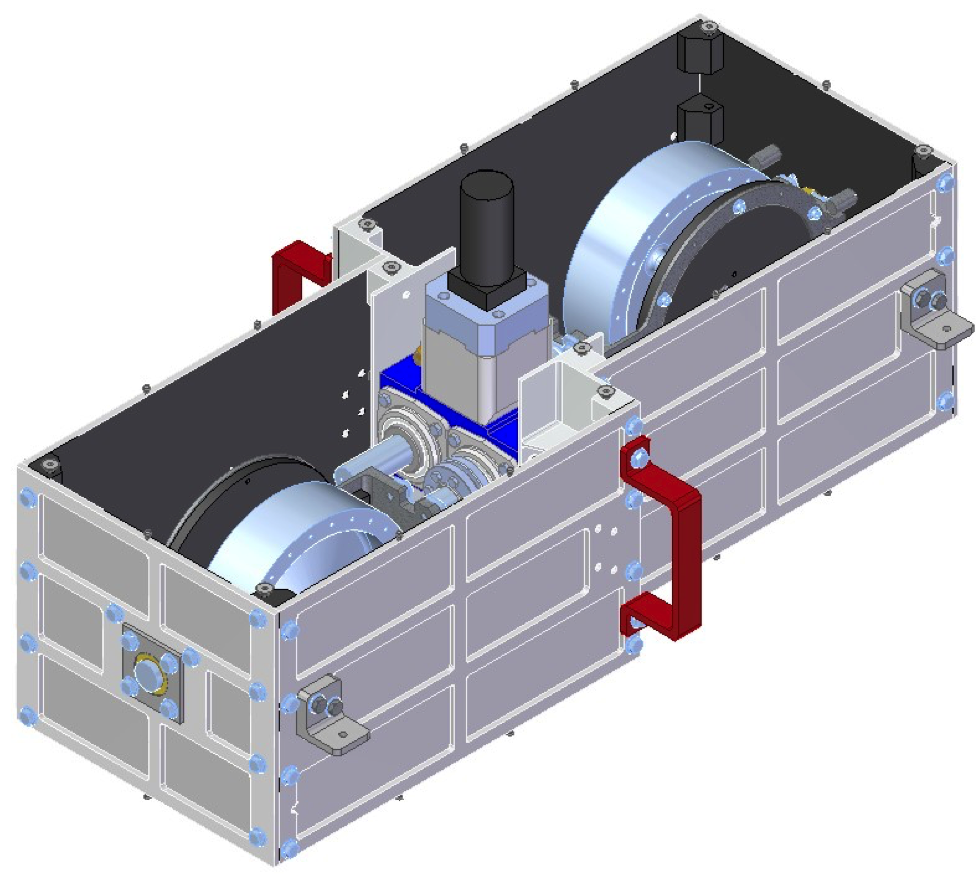
\includegraphics[width=\textwidth]{Figures/CCMG-case.png}
	\caption{}
	\label{fig:CCMGcase}
    \end{figure}


\subsection{Momentum dump mechanism}
\label{subsec:chap3momdumpmotor}

\begin{figure}[!ht]
	\centering
	\includestandalone{Figures/rotator}
	\caption[Momentum dump assembly]{Momentum dump assembly}
	\label{fig:rotator}
    \end{figure}


\subsection{Elevation control (Rotators)}
\subsection{Delay lines}
\subsection{Tip/tilt}
\subsection{Fine guidance sensor}


\subsection{Control electronics}
Clocks and timings \\
Computers
\subsection{Software architecture}
